% Part V — Summary and Key Takeaways
\section{Summary and Key Takeaways}

% Slide 13 — Summary Table
\begin{frame}{MLE vs MoM Summary}
  \begin{center}
    \footnotesize
    \begin{tabular}{|l|l|l|}
    \hline
    \textbf{Property} & \textbf{MLE} & \textbf{MoM} \\
    \hline
    Existence & Requires likelihood & Requires finite moments \\
    \hline
    Computation & Optimization required & Simple equations \\
    \hline
    Consistency & Yes & Yes \\
    \hline
    Asymptotic Normality & Yes & Yes \\
    \hline
    Efficiency & Asymptotically efficient & Not efficient in general \\
    \hline
    Robustness & Moderate & Sensitive to outliers \\
    \hline
    Invariance & Yes & No \\
    \hline
    \end{tabular}
  \end{center}

  \vspace{1em}
  \begin{center}
  \begin{adjustbox}{max height=0.40\textheight}
    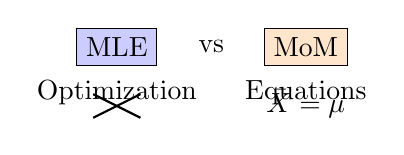
\begin{tikzpicture}[scale=0.6]
      % MLE = optimization
      \node[draw, rectangle, fill=blue!20] at (-2, 0) {MLE};
      \node[below] at (-2, -0.5) {Optimization};
      \draw[thick] (-2.5, -1) -- (-1.5, -1.5);
      \draw[thick] (-1.5, -1) -- (-2.5, -1.5);

      % vs
      \node at (0, 0) {vs};

      % MoM = equations
      \node[draw, rectangle, fill=orange!20] at (2, 0) {MoM};
      \node[below] at (2, -0.5) {Equations};
      \node at (2, -1.2) {$\bar{X} = \mu$};
    \end{tikzpicture}
    \end{adjustbox}
  \end{center}
\end{frame}

% Slide 14 — Big Picture
\begin{frame}{Key Takeaways}
  \begin{itemize}
    \item \textbf{Good estimator} = balance bias and variance
    \item Both MLE and MoM are consistent and asymptotically normal
    \item \textbf{MLE} = gold standard in large samples
    \item \textbf{MoM} = simple first approach
    \item Choosing an estimator depends on context:
    \begin{itemize}
      \item Data size
      \item Model complexity
      \item Robustness requirements
    \end{itemize}
  \end{itemize}

  \vspace{1em}
  \begin{center}
    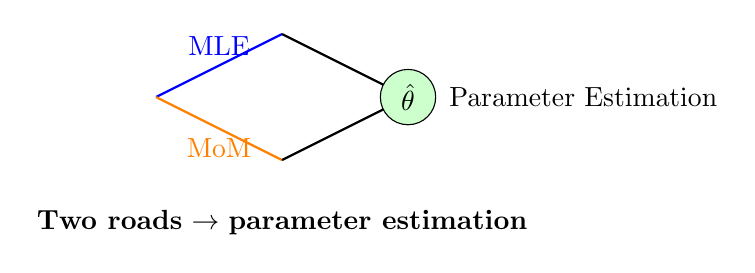
\begin{tikzpicture}[scale=0.8]
      % Two roads
      \draw[thick, blue] (0, 0) -- (2, 1);
      \node[blue, above] at (1, 0.5) {MLE};

      \draw[thick, orange] (0, 0) -- (2, -1);
      \node[orange, below] at (1, -0.5) {MoM};

      % Converging to parameter estimation
      \draw[thick] (2, 1) -- (4, 0);
      \draw[thick] (2, -1) -- (4, 0);

      \node[draw, circle, fill=green!20] at (4, 0) {$\hat{\theta}$};
      \node[right] at (4.5, 0) {Parameter Estimation};

  \node at (2, -2) {\textbf{Two roads} \(\to\) \textbf{parameter estimation}};
    \end{tikzpicture}
  \end{center}
\end{frame}